\documentclass[french,12pt]{article}



%%%%%%%%%%%%%%%%%%%%%%%%%%%%%%%%%%%%%%%%%%%%%%%%%%%%%%%%%%%%%%%%
%%%%%%%%%%%%%%%%%%%%%%%%%%%%%%%%%%%%%%%%%%%%%%%%%%%%%%%%%%%%%%%%
%%%%%%%%%%%%%%%%%%%%%%%%%%%%%%%%%%%%%%%%%%%%%%%%%%%%%%%%%%%%%%%%

\begin{document}


%%%%%%%%%%%%%%%%%%%%%%%%%%%%%%%%%%%%%%%%%%%%%%%%%%%%%%%%%%%%%%%%
%%%%%%%%%%%%%%%%%%%%%%%%%%%%%%%%%%%%%%%%%%%%%%%%%%%%%%%%%%%%%%%%
%%%%%%%%%%%%%%%%%%%%%%%%%%%%%%%%%%%%%%%%%%%%%%%%%%%%%%%%%%%%%%%%

\part{Présentation générale du problème}

\section{Projet}

\subsection{Finalité}

L'objectif de ce projet est de créer une base de données géo-référencées. Cette base est destinée à constituer un rassemblement volumineux de données géographiques sur le territoire. Les données sont rapatriées de sources diverses puis traitées automatiquement. Enfin, elle sont importées dans la base.

À des fins d'études recroisant ces données, cette base est vouée à être un source de données commune à de multiples utilisateurs. Dans cette optique, cette base sera munie d'un ensemble de requêtes basiques, c'est-à-dire de filtres larges permettant une utilisation facilitée de ces données par des logiciels de traitements, en aval.

\subsection{Problématique}

À l'\bsc{IFSTTAR}, certaines recherches requièrent la manipulation de données géographiques~: statistiques, recroisements, simulations. Actuellement le regroupement, stockage, filtrage, et partage de ces données est réalisé manuellement. Par conséquent, les mêmes manipulations sont souvent répétées, ce qui constitue une perte d'efforts et de temps.

\subsection{Énoncé du besoin}

Le travail à effectuer vise à créer un serveur de données centralisé en important automatiquement des données, en les pré-traitant, puis en les rapatriant dans la base.

L'utilisateur doit pouvoir définir l'ensembles paramètres d'exécution avant le lancement. Ainsi, sans modifier le code source, il doit être en mesure de spécifier les éléments énoncés ci-dessous.

\begin{description}
  \item[comportement~:] réaction du programme à une situation donnée (exemple~: niveau de verbosité)
  \item[structure de la base~:] tables, attributs, clés, relations, contraintes
  \item[données~:] source des données et traitements attendus (exemple~: spécifier la table qui va accueillir un ensemble de données)
\end{description}

L'ensemble de ces spécifications s'effectueront à travers des fichiers de configuration, de format \bsc{JSON}. Toute interaction entre le logiciel et l'utilisateur s'effectuera par ces fichiers. Ainsi, l'utilisateur n'aura pas besoin d'altérer le code source pour contrôler le comportement du logiciel.

De plus, seuls les paramètres absolument nécessaires seront à préciser, comme par exemple la structure de la base si l'utilisateur souhaite la créer. L'utilisateur aura bien entendu la liberté de redéfinir les autres paramètres au cas où leurs valeurs par défaut ne lui conviennent pas.

\subsection{Solution apportée}

Pour répondre au besoin énoncé ci-dessus, une base de données centralisée ainsi que des procédures d'importation, de nettoyage, et de traitement de données sont crées. L'ensemble de ces solutions permet notamment~:

\begin{itemize}
  \item un stockage massif performant de données
  \item l'élimination des tâches de pré-traitement~: récupération, nettoyage, uniformisation, recherche de liens (clés \& relations)
  \item la mutualisation des données, rendues accessibles à de multiples utilisateurs
  \item la mise à disposition de requêtes basiques de sélection avec application de filtres (attributaires, géographiques)
\end{itemize}

\subsection{Planification}

Diagramme de Gantt~:

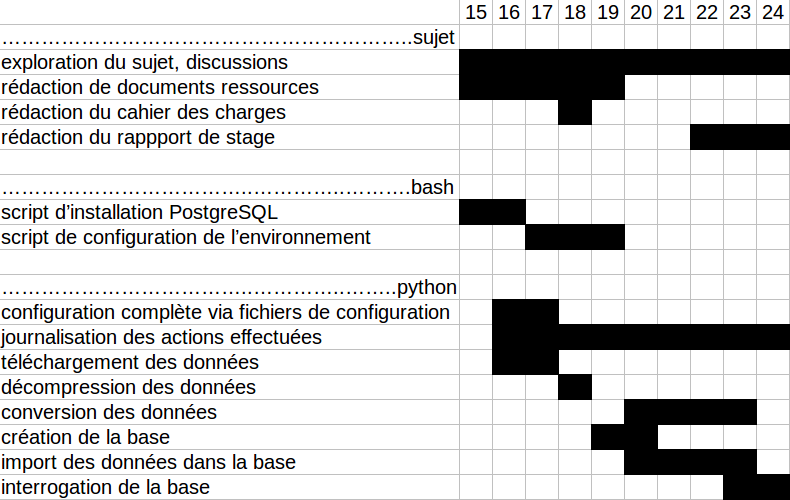
\includegraphics[height=25em]{gantt}

\section{Contexte}

\subsection{Études déjà effectuées}

Marc \bsc{Noël} a d'ores-et-déjà effectué un travail préliminaire sur les données et établi les liens existants. En effet, en parcourant et effectuant des traitements sur ces données il a pu conçevoir le schéma de la base de données.

C'est ce schéma qu'il revient ici d'implémenter, en discutant des adaptations mineures éventuelles. Ce schéma se veut proche des données d'entrée. De cette manière, l'intégration des données est facilitée.

\subsection{Nature des prestations demandées}

En premier lieu, le développement de deux scripts shell (\texttt{bash}). Ces scripts, non interactifs, vont venir préparer l'exécution ultérieure du code \texttt{Python}. En effet, ils se chargent de d'installer et configurer automatiquement l'ensemble des composants de l'environnement. Le premier se charge d'installer et de configurer la base \texttt{PostgreSQL}. Le second se charge de préparer l'exécution du code \texttt{Python} en installant les dépendances (les packages) auxquels il fait appel.

En second lieu, le développement d'un script \texttt{Python} chargé de manipuler les données. Ce dernier doit effectuer un ensemble de traitements tels que précisés par l'utilisateur.

\subsection{Parties concernées par le déroulement du projet et ses résultats}

En ce qui concerne l'\bsc{IUT} informatique de Nantes, Monsieur Loïg \bsc{Jezequel}, est chargé en tant qu'enseignant référent de suivre et évaluer ce stage. Ce suivi est réalisé via un message électronique envoyé en chaque fin de semaine, ainsi qu'une visite sur le lieu de stage. De même, plusieurs rendus sont à fournir tel qu'un résumé du sujet, ce cahier des charges, ainsi que le rapport de stage.

En ce qui concerne la structure d'accueil, l'\bsc{IFSTTAR}, Pascal \bsc{Gastineau} et Pierre \bsc{Hankach} jouent le rôle de tuteurs. Ils seront également les commanditaires et les clients du développement effectué.

Enfin, une soutenance ponctue le stage. Le jury sera alors composé de Pierre \bsc{Hankach}, Loïg \bsc{Jezequel}, ainsi qu'un second professeur de l'\bsc{IUT}.

\part{Détail technique du besoin}

\section{Étapes préliminaires~: scripts shell}

\subsection{Installation et configuration de \texttt{PostgreSQL}}

En premier lieu, le rôle de ce script est d'installer \texttt{PostgreSQL} et l'extension \texttt{PostGIS}.

En second lieu, ce script a pour rôle de configurer \texttt{PostgreSQL}. Cela est réalisé via l'édition automatisée de fichiers de configuration, et permet l'obtention des fonctionnalités suivantes~:

\begin{description}
  \item[compatibilité~:] support \bsc{UTF-8} pour la base \texttt{template1}
  \item[rôles~:] création de deux rôles (groupes) distincts permettant l'un la lecture et l'autre écriture ; ils seront hérités par les utilisateurs créés manuellement à posteriori
  \item[création~:] création de la base qui recevra les données
  \item[sécurité~:] ajout d'un mot de passe pour l'utilisateur \texttt{postgres}
  \item[journalisation~:] connexions et déconnexions
  \item[authentification] définition de la politique de sécurité
  \item[connexions~:] autorisation des connexions à distance
\end{description}

\subsection{Préparation de l'environnement d'exécution}

Le rôle de ce script est de préparer l'environnement d'exécution. Sa tâche principale est d'effectuer une installation de \texttt{miniconda} et d'importer un l'environnement adéquat. Cet environnement aura été préalablement exporté et conservé dans l'arborescence du projet.

\section{Applicatif \texttt{Python}}

\subsection{Description fonctionnelle}

Le code \texttt{Python} devra fournir les fonctionnalités suivantes~:

\begin{itemize}
  \item configuration complète via fichiers de configuration
  \item journalisation des actions effectuées
  \item téléchargement des données
  \item décompression des données
  \item conversion des données
  \item création de la base
  \item import des données dans la base
  \item interrogation de la base
\end{itemize}

\subsection{Modularité, découpage en sous-ensembles}

Le découpage en sous-ensembles s'articule autour de modules. Chaque module regroupe un ensemble logique de fonctionnalités. La figure suivante montre l'arbre décrivant une structure possible du projet.

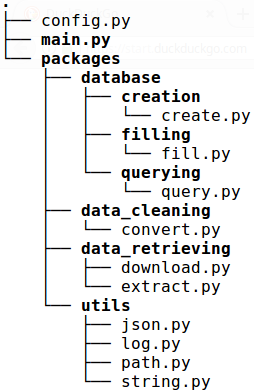
\includegraphics[height=15em]{arborescence}

Cette structure n'est pas définitive. En effet, elle est sujette à être étoffée ou redécoupée si nécessaire. Cependant, le découpage montrera toujours clairement les différentes tâches, de manière à les séparer. En effet les modules de plus haut niveau correspondent aux tâches principales de l'application.

%%%%%%%%%%%%%%%%%%%%%%%%%%%%%%%%%%%%%%%%%%%%%%%%%%%%%%%%%%%%%%%%
%%%%%%%%%%%%%%%%%%%%%%%%%%%%%%%%%%%%%%%%%%%%%%%%%%%%%%%%%%%%%%%%
%%%%%%%%%%%%%%%%%%%%%%%%%%%%%%%%%%%%%%%%%%%%%%%%%%%%%%%%%%%%%%%%

\end{document}
